

%! When the figure is used in the title, the figure environment is removed

%\begin{figure*}[h!]
%    \centering
    %\includegraphics[width=0.87\linewidth]{aper_yeye.jpg}
    %* Figure
    % for the use in the online editor: \usepackage{tikz} 
    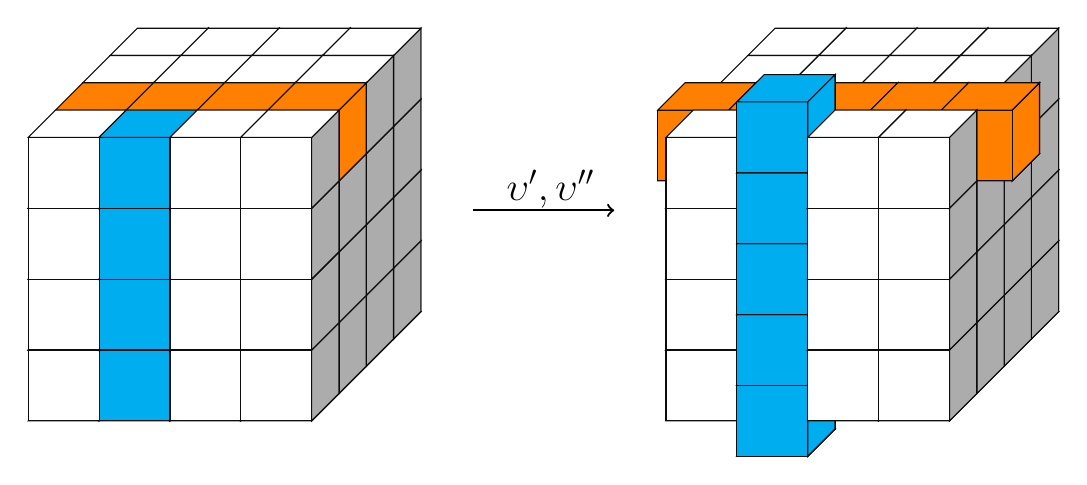
\begin{tikzpicture}[scale=0.9] %! The original scale is 1
        % Define the tile
        \def\tile{
        % Draw the unit cube
            \draw[black!95] (1,0,0) -- (1,0,1) -- (1,1,1) -- (1,1,0) -- cycle; % left face
            \draw[black!95] (0,0,0) -- (1,0,0) -- (1,0,1) -- (0,0,1) -- cycle; % bottom face
            \draw[black!95] (0,0,0) -- (0,1,0) -- (1,1,0) -- (1,0,0) -- cycle; % back face
            \draw[black!95, fill=gray!65] (1,0,0) -- (1,1,0) -- (1,1,1) -- (1,0,1) -- cycle; % right face
            \draw[black!95, fill=white] (0,0,1) -- (1,0,1) -- (1,1,1) -- (0,1,1) -- cycle; % front face
            \draw[black!95, fill=white](0,1,0) -- (0,1,1) -- (1,1,1) -- (1,1,0) -- cycle; % top face
        }

        \def\tilecolumn{
            % Draw the unit cube
                \draw[black!95] (1,0,0) -- (1,0,1) -- (1,1,1) -- (1,1,0) -- cycle; % left face
                \draw[black!95] (0,0,0) -- (1,0,0) -- (1,0,1) -- (0,0,1) -- cycle; % bottom face
                \draw[black!95] (0,0,0) -- (0,1,0) -- (1,1,0) -- (1,0,0) -- cycle; % back face
                \draw[black!95, fill=cyan] (1,0,0) -- (1,1,0) -- (1,1,1) -- (1,0,1) -- cycle; % right face
                \draw[black!95, fill=cyan] (0,0,1) -- (1,0,1) -- (1,1,1) -- (0,1,1) -- cycle; % front face
                \draw[black!95, fill=cyan](0,1,0) -- (0,1,1) -- (1,1,1) -- (1,1,0) -- cycle; % top face
            }
        
        \def\tilerow{
            % Draw the unit cube
                \draw[black!95] (1,0,0) -- (1,0,1) -- (1,1,1) -- (1,1,0) -- cycle; % left face
                \draw[black!95] (0,0,0) -- (1,0,0) -- (1,0,1) -- (0,0,1) -- cycle; % bottom face
                \draw[black!95] (0,0,0) -- (0,1,0) -- (1,1,0) -- (1,0,0) -- cycle; % back face
                \draw[black!95, fill=orange] (1,0,0) -- (1,1,0) -- (1,1,1) -- (1,0,1) -- cycle; % right face
                \draw[black!95, fill=orange] (0,0,1) -- (1,0,1) -- (1,1,1) -- (0,1,1) -- cycle; % front face
                \draw[black!95, fill=orange](0,1,0) -- (0,1,1) -- (1,1,1) -- (1,1,0) -- cycle; % top face
            }
    
        % Draw the tiling pattern LEFT: x = 0,1,2,3
        % not shifted
        % the backseat boys
        \foreach \x in {0,1,2,3}{
            \foreach \y in {-2,-1,0,1}{
                \foreach \z in {-2,-1}{
                    \pgfmathsetmacro{\shiftX}{\x}
                    \pgfmathsetmacro{\shiftY}{\y}
                    \pgfmathsetmacro{\shiftZ}{\z}
                    
                    \begin{scope}[shift={(\shiftX,\shiftY,\shiftZ)}]
                    \tile % Draw the tile
                    \end{scope}
                }
            }
        }
        % Draw the back four cubes as two rows for the shift in X
        % not shifted
        \foreach \x in {0,1,2,3}{
            \foreach \y in {-2,-1,0}{
                \foreach \z in {0}{
                    \pgfmathsetmacro{\shiftX}{\x}
                    \pgfmathsetmacro{\shiftY}{\y}
                    \pgfmathsetmacro{\shiftZ}{\z}
                    
                    \begin{scope}[shift={(\shiftX,\shiftY,\shiftZ)}]
                    \tile % Draw the tile
                    \end{scope}
                }
            }
        }
        % Will be shifted – in the X direction
        \foreach \x in {0,1,2,3}{
            \foreach \y in {1}{
                \foreach \z in {0}{
                    \pgfmathsetmacro{\shiftX}{\x}
                    \pgfmathsetmacro{\shiftY}{\y}
                    \pgfmathsetmacro{\shiftZ}{\z}
                    
                    \begin{scope}[shift={(\shiftX,\shiftY,\shiftZ)}]
                    \tilerow % Draw the tile
                    \end{scope}
                }
            }
        }
        
        
        % not shifted
        \foreach \x in {0}{
            \foreach \y in {-2,-1,0,1}{
                \foreach \z in {1}{
                    \pgfmathsetmacro{\shiftX}{\x}
                    \pgfmathsetmacro{\shiftY}{\y}
                    \pgfmathsetmacro{\shiftZ}{\z}
                    
                    \begin{scope}[shift={(\shiftX,\shiftY,\shiftZ)}]
                    \tile % Draw the tile
                    \end{scope}
                }
            }
        }
        % Draw the front four cubes as two columns for the shift in Y
        % Will be shifted – in the Y direction
        \foreach \x in {1}{
            \foreach \y in {-2,-1,0,1}{
                \foreach \z in {1}{
                    \pgfmathsetmacro{\shiftX}{\x}
                    \pgfmathsetmacro{\shiftY}{\y}
                    \pgfmathsetmacro{\shiftZ}{\z}
                    
                    \begin{scope}[shift={(\shiftX,\shiftY,\shiftZ)}]
                    \tilecolumn % Draw the tile
                    \end{scope}
                }
            }
        }
        % not shifted
        \foreach \x in {2,3}{
            \foreach \y in {-2,-1,0,1}{
                \foreach \z in {1}{
                    \pgfmathsetmacro{\shiftX}{\x}
                    \pgfmathsetmacro{\shiftY}{\y}
                    \pgfmathsetmacro{\shiftZ}{\z}
                    
                    \begin{scope}[shift={(\shiftX,\shiftY,\shiftZ)}]
                    \tile % Draw the tile
                    \end{scope}
                }
            }
        }
        
        % Draw the Inbetween stuff
        %———————————————————————————————————
        \draw[->, thick, black] (5.5,0.2) -- (7.5,0.2);
        \node[black] at (6.6,0.5) {\Large $\upsilon',\upsilon''$}; 
        
        
        
        
        % Draw the tiling pattern RIGHT: x= 9,10,11,12
        %———————————————————————————————————
        % not shifted
        % the backseat boys
        \foreach \x in {9,10,11,12}{
            \foreach \y in {-2,-1,0,1}{
                \foreach \z in {-2,-1}{
                    \pgfmathsetmacro{\shiftX}{\x}
                    \pgfmathsetmacro{\shiftY}{\y}
                    \pgfmathsetmacro{\shiftZ}{\z}
                    
                    \begin{scope}[shift={(\shiftX,\shiftY,\shiftZ)}]
                    \tile % Draw the tile
                    \end{scope}
                }
            }
        }
        % Draw the back four cubes as two rows for the shift in X
        % not shifted
        \foreach \x in {9,10,11,12}{
            \foreach \y in {-2,-1,0}{
                \foreach \z in {0}{
                    \pgfmathsetmacro{\shiftX}{\x}
                    \pgfmathsetmacro{\shiftY}{\y}
                    \pgfmathsetmacro{\shiftZ}{\z}
                    
                    \begin{scope}[shift={(\shiftX,\shiftY,\shiftZ)}]
                    \tile % Draw the tile
                    \end{scope}
                }
            }
        }
        % Will be shifted – in the X direction
        \foreach \x in {8,9,10,11,12}{
            \foreach \y in {1}{
                \foreach \z in {0}{
                    \pgfmathsetmacro{\shiftX}{\x+0.5}
                    \pgfmathsetmacro{\shiftY}{\y}
                    \pgfmathsetmacro{\shiftZ}{\z}
                    
                    \begin{scope}[shift={(\shiftX,\shiftY,\shiftZ)}]
                    \tilerow % Draw the tile
                    \end{scope}
                    
                    %\ifnum\x=9
                    %    \draw[->, orange] (\shiftX+1,1.4) --node[below] {$0.5$} (\shiftX+2,1.4);             \fi
                }
            }
        }
        

        % not shifted
        \foreach \x in {9}{
            \foreach \y in {-2,-1,0,1}{
                \foreach \z in {1}{
                    \pgfmathsetmacro{\shiftX}{\x}
                    \pgfmathsetmacro{\shiftY}{\y}
                    \pgfmathsetmacro{\shiftZ}{\z}
                    
                    \begin{scope}[shift={(\shiftX,\shiftY,\shiftZ)}]
                    \tile % Draw the tile
                    \end{scope}
                }
            }
        }
        % Draw the front four cubes as two columns for the shift in Y
        % Will be shifted – in the Y direction
        \foreach \x in {10}{
            \foreach \y in {-3,-2,-1,0,1}{
                \foreach \z in {1}{
                    \pgfmathsetmacro{\shiftX}{\x}
                    \pgfmathsetmacro{\shiftY}{\y+0.5}
                    \pgfmathsetmacro{\shiftZ}{\z}
                    
                    \begin{scope}[shift={(\shiftX,\shiftY,\shiftZ)}]
                    \tilecolumn % Draw the tile
                    \end{scope}
                    
                    %\ifnum\y=1
                    %    \draw[->, thick, cyan] (7,\shiftY+0.5) --node[right] {$0.5$} (7,\shiftY+1.5);             \fi
                }
            }
        }
        % not shifted
        \foreach \x in {11,12}{
            \foreach \y in {-2,-1,0,1}{
                \foreach \z in {1}{
                    \pgfmathsetmacro{\shiftX}{\x}
                    \pgfmathsetmacro{\shiftY}{\y}
                    \pgfmathsetmacro{\shiftZ}{\z}
                    
                    \begin{scope}[shift={(\shiftX,\shiftY,\shiftZ)}]
                    \tile % Draw the tile
                    \end{scope}
                }
            }
        }
        
        
  
    \end{tikzpicture}
    %\caption{Illisustrated in the \cref{fig:big_aperi} is simply a bigger version of the aperiodic tile we have constructed.}
    %\label{fig:big_aperi}
%\end{figure*}
